\documentclass[10pt]{article}
% Эта строка — комментарий, она не будет показана в выходном файле
\usepackage{ucs}
\usepackage[utf8x]{inputenc} % Включаем поддержку UTF8
\usepackage[russian]{babel}  % Включаем пакет для поддержки русского языка
\usepackage{amsmath}
\usepackage{amssymb}
\usepackage{mathtools}

\hoffset=0mm
\voffset=0mm
\textwidth=170mm        % ширина текста
\oddsidemargin=-0mm   % левое поле 25.4 - 5.4 = 20 мм
\textheight=240mm       % высота текста 297 (A4) - 40
\topmargin=-15.4mm      % верхнее поле (10мм)
\headheight=5mm      % место для колонтитула
\headsep=5mm          % отступ после колонтитула
\footskip=8mm         % отступ до нижнего колонтитула



% \textwidth=180mm    
% \oddsidemargin=-10mm 

\title{Лабораторная работа № 2.2.6: {\it Определение энергии активации по температурной зависимости вязкости жидкости.}}
\author{Зотов Алексей, 497}
\date{\today}

\begin{document}

\maketitle
\textbf{Цель работы:}
    \begin{enumerate}
    \item Измерение скорости падения шариков при разной температуре жидкости.
    \item Вычисление вязкости жидкости по закону Стокса и рассчет энергии активации.
    \end{enumerate}

\textbf{В работе испольуются:} Стеклянный цилиндр с исследуемой жидкостью (глицерин); термостат; секундомер; микроскоп; мелкие стеклянные и стальные шарики(диаметром около 1 мм).

\textbf{Теория.}
Молекулы, медленно перемещаясь внутри жизкости, пребывая часть времени около определённых мест равновесия и образуя картину меняющейся со временем пространственной решётки. Для перехода в новое состояние, молекула должна преодолеть участки с большой потенциальной 
энергией, превышающей среднюю энергию молекул. Для этого тепловая энергия молекул должна увеличиться на величину $W$, называемую энергией активации.


\begin{equation}
    \eta \sim A e^{W/kT}
\end{equation}

Энергию активации молекулы жидкости можно получить, отложив $y(\frac{1}{T}) = \ln \eta $, как угловой коэффициент получившейся прямой.

Для исследования температурной зависимотси вязкости жидкости используется метод Стокса, основанный на измерении скорости свободного падения шарика в жидкости.

При ламинарном обтекании шарика безграничной жидкостью, сила сопротивления выражается как:

\begin{equation}
    F = 6 \pi \eta r v
\end{equation}

На шарик действуют три силы: сила тяжести, архимедова сила, сила вязкости, зависящая от скорости. Тогда уравнение движения шарика в жидкости по второму закону Ньютона выглядит как:

\begin{equation}
    V g (\rho - \rho_{lq} ) - 6 \pi \eta r v = V \rho \frac{dv}{dt}
\end{equation}

где $V$ — объем шарика, $\rho$ — его плотность, $\rho_{lq}$ — плотность жидкости, $g$ — ускорение свободного падения.

Отсюда находим:

\begin{equation}
    v(t) = v_{st} - [v_{st} - v(0)] e^{-t/ \tau}
\end{equation}

Где $v(0)$ - скорость шарика в момент начала его движения, $v_{st}$ - установившаяся скорость, $\tau$ - время релаксации.

\begin{equation}
    v_{st} = \frac{V g (\rho - \rho_{lq} )}{6 \pi \eta r v}
    = \frac{2}{9} g r^2 \frac{(\rho - \rho_{lq} )}{\eta}, 
    \quad 
    \tau = \frac{V \rho}{6 \pi \eta r v} = \frac{2 r^2 \rho}{9 \eta}
\end{equation}
{\small
Как видно, скорость шарика экспоненциально приближается к установившейся скорости. Установление скорости определяется величиной $\tau$, имеющей размерность времени и называющейся временем релаксации. Если вре
мя падения в несколько раз больше времени релаксации, процесс установления скорости можно считать закончившимся.
}
Измеряя на опыте установившуюся скорость, можно определить вязкость жидкости по формуле:

\begin{equation}
    \eta = \frac{2}{9} g r^2 \frac{(\rho - \rho_{lq} )}{v_{st}}
\end{equation}

\newpage
\textbf{Экспериментальная установка}

% \begin{figure}[htp]
    \begin{center}
    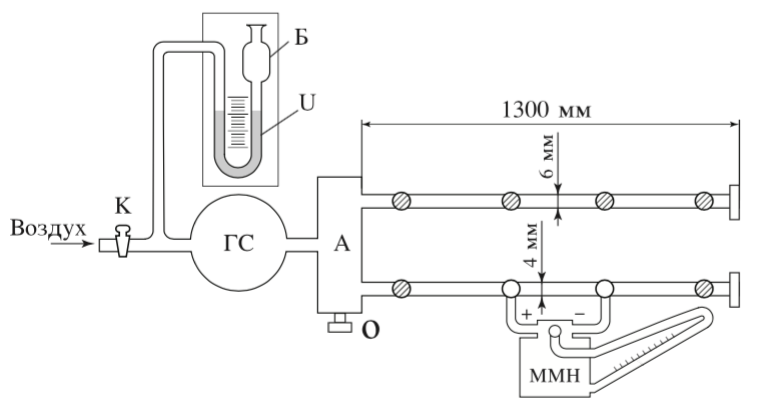
\includegraphics[width=5cm]{ust.png} \\Схема установки
    \end{center}

$L_1 = L_2 = 10$см.
% \end{figure}

% \newpage
\textbf{Применимость формулы Стокса}

Определим характер обтекания:
\begin{equation}
    Re = \frac{vr \rho_{lq}}{\eta}
\end{equation}

Обтекание является ламинарным при $Re < 10$

Определим также допустимое расстояние между границей жидкости и верхней меткой:

\begin{equation}
    S = v_{st} \tau (\frac{t}{\tau} - 1 + e^{-t/\tau})
\end{equation}

\textbf{Ход работы.}
Будем считать $v_{st} = \frac{L}{t_2 - t_1}$ , то есть как скорость на втором участке.\\
Определим погрешность:
\begin{equation}
    (\frac{\sigma_\eta}{\eta})^2 = 2^2(\frac{\sigma_r}{r})^2 +  (\frac{\sigma_t}{t})^2 + \varepsilon^2_{\rho_{gl}}
\end{equation} 
$\varepsilon_{\rho_{gl}} = 0.05$, $\sigma_{dx}= 0.05 $ мм , $\sigma_t= 0.1$ с,$\sigma_T= 0.1 C^o$ .

Из (1) получим:
\begin{equation} 
    \ln \eta = \frac{W}{k} \cdot \frac{1}{T} + \text{const}
\end{equation}
тогда $W = a \cdot k$ , где $ax + b$ - зависимость $\ln \eta (x = \frac{1}{T})$

Найдем $а$:
\begin{equation}
    a = \left < \frac{\Delta y_i}{\Delta x_i} \right > , y_i = \ln \eta_i , x_i = \frac{1}{T_i}
\end{equation}

\begin{equation}
    \sigma_a = \frac{1}{n} \sqrt{ \sum \sigma^2 \left(\frac{\Delta y_i}{\Delta x_i} \right)}
\end{equation}

\begin{equation}
    \varepsilon^2_{\frac{\Delta y}{\Delta x}} = \varepsilon^2_{\Delta y} + \varepsilon^2_{\Delta x}
\end{equation}

\begin{enumerate}
    \item \underline{Стеклянные шарики.} \\
    $\rho = \rho_{\text{ст}} = 2.5 \text{г}/\text{см}^3$
    % \begin{center}
    \begin{table}[htp]
                    Стеклянные шарики\\
                    \begin{tabular}{|c|c|c|c|c|c|c|c|c|c|c|c|c|c|}
                            \hline
                                $ T , C^o$  &20.6 &20.6 &25.0 &29.8 &29.8 &34.9 &34.9 &40.4 &40.4 &45.0 &45.0 &50.0 &50.0 \\
                            \hline
                                $ t_1 , c$   &15.2 &15.5 &13.6 &9.9 &9.4 &6.2 &6.3 &4.6 &4.7 &3.7 &3.3 &2.9 &2.8\\
                            \hline
                                $ t_2 , c$ &30.9 &31.4 &27.2 &20.0 &18.8 &11.9 &12.2 &8.7 &8.7 &7.2 &6.7 &5.9 &5.6\\
                            \hline
                                $ dx, mm, $ &0.8 &0.77 &0.9 &0.83 &0.85 &0.9 &0.83 &0.8 &0.75 &0.73 &0.7 &0.7 &0.7 \\
                            \hline
                                $v_{st}, cm/c$ &0.64 &0.63 &0.74 &0.99 &1.06 &1.75 &1.69 &2.44 &2.5 &2.86 &2.94 &3.33 &3.57 \\
                            \hline
                                $\rho_{gl} g/cm^3$, &1.263 &1.263 &1.26 &1.258 &1.258 &1.254 &1.254 &1.251 &1.251 &1.248 &1.248 &1.245 &1.245 \\ 
                            \hline
                                $\eta , \text{мПа} \cdot c$ &1777.4 &1713.3 &1619.6 &1148.1 &1175.3 &618.7 &640.4 &468.7 &435.2 &420.8 &408.8 &344.6 &337.5 \\
                            \hline
                                $\sigma_{\eta} , \text{мПа} \cdot c$ &124.7 &121.6 &112.5 &81.0 &81.2 &45.1 &46.6 &34.7 &32.6 &31.4 &30.7 &26.7 &26.2 \\
                            \hline
                                $\varepsilon_{\eta}$ &0.07 &0.071 &0.069  &0.071 &0.069 &0.073 &0.073 &0.074 &0.075 &0.075 &0.075 &0.077 &0.078 \\
                            \hline
                                $S_{\tau}$, см &0.131 &0.13 &0.151 &0.203 &0.219 &0.359 &0.347 &0.498 &0.511 &0.582 &0.599 &0.678 &0.726 \\
                            \hline
                                $Re$ &0.1 &0.1 &0.1 &0.2 &0.2 &0.7 &0.7 &1.3 &1.4 &1.8 &1.9 &2.5 &2.8\\
                                \hline
                        \end{tabular}
    \end{table}
    \begin{center}
    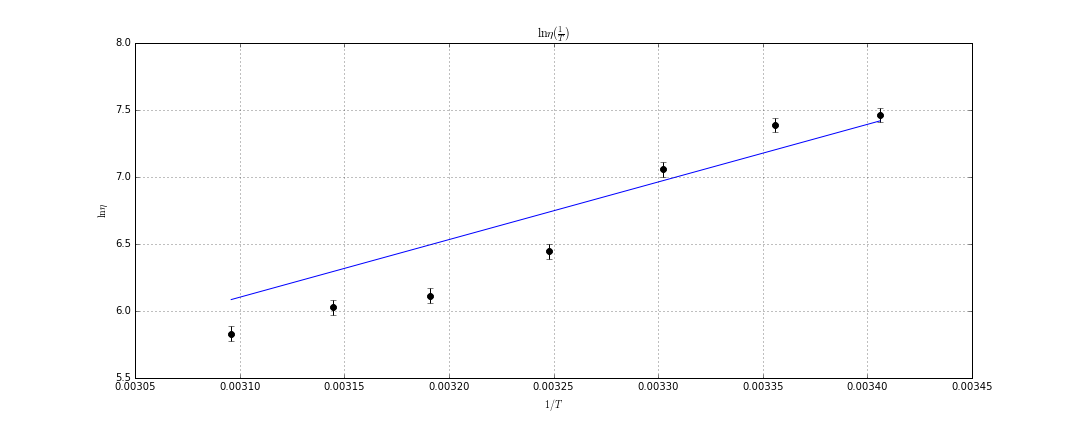
\includegraphics[width=18cm]{g1.png} 
    \end{center}

    $\sigma_{tg \alpha} = 124.6 , \varepsilon_{tg \alpha} = 0.024$ \\
    $\tg \alpha \approx 5104.87 \implies W = (7.05 \pm 0.17)* 10^{-20}$ [Дж] $\approx 0.44$ [эВ].

    \item \underline{Металлические шарики.}
        $\rho = \rho_{\text{ir}} = 7.8 \text{г}/\text{см}^3$
        \begin{table}[htp]
                    Металлические шарики\\
                    \begin{tabular}{|c|c|c|c|c|c|c|c|c|c|c|c|c|c|}
                            \hline
                                $ T , C^o$  &21.7 &24.9 &25.0 &30.0 &30.0 &34.9 &35.0 &40.3 &40.4 &45.0 &45.0 &50.0 &50.0 \\
                            \hline
                                $ t_1 , c$   &21.6 &18.6 &14.6 &10.0 &9.3 &6.0 &7.9 &4.9 &6.7 &4.6 &6.2 &4.7 &3.4 \\
                            \hline
                                $ t_2 , c$ &43.2 &36.0 &29.3 &20.8 &19.5 &12.3 &14.5 &10.3 &13.6 &10.1 &12.1 &9.5 &6.8 \\
                            \hline
                                $ dx, mm, $ &0.8 &0.77 &0.9 &0.83 &0.85 &0.9 &0.83 &0.8 &0.75 &0.73 &0.7 &0.7 &0.7 \\
                            \hline
                                $v_{st}, cm/c$ &0.46 &0.57 &0.68 &0.93 &0.98 &1.59 &1.52 &1.85 &1.45 &1.82 &1.69 &2.08 &2.94 \\
                            \hline
                                $\rho_{gl} g/cm^3$, &1.262 &1.26 &1.26 &1.257 &1.257 &1.254 &1.254 &1.251 &1.251 &1.248 &1.248 &1.245 &1.245 \\
                            \hline
                                $\eta , \text{мПа} \cdot c$ &1968.3 &1469.3 &1695.9 &1060.2 &1050.1 &727.5 &648.2 &492.9 &553.6 &418.2 &412.5 &335.8 &237.8 \\
                            \hline
                                $\sigma_{\eta} , \text{мПа} \cdot c$ &265.1 &204.7 &207.0 &138.6 &134.6 &89.4 &85.1 &67.0 &79.2 &61.5 &62.8 &51.3 &36.7 \\
                            \hline
                                $\varepsilon_{\eta}$ &0.135 &0.139 &0.122 &0.131 &0.128 &0.123 &0.131 &0.136 &0.143 &0.147 &0.152 &0.153 &0.154 \\
                            \hline
                                $S_{\tau}$, см &0.056 &0.07 &0.083 &0.113 &0.119 &0.193 &0.184 &0.225 &0.176 &0.221 &0.206 &0.253 &0.357 \\
                            \hline
                                $Re$ &0.0 &0.0 &0.0 &0.1 &0.1 &0.2 &0.2 &0.4 &0.2 &0.4 &0.4 &0.5 &1.1 \\
                                \hline
                        \end{tabular}
    \end{table}
    \begin{center}
    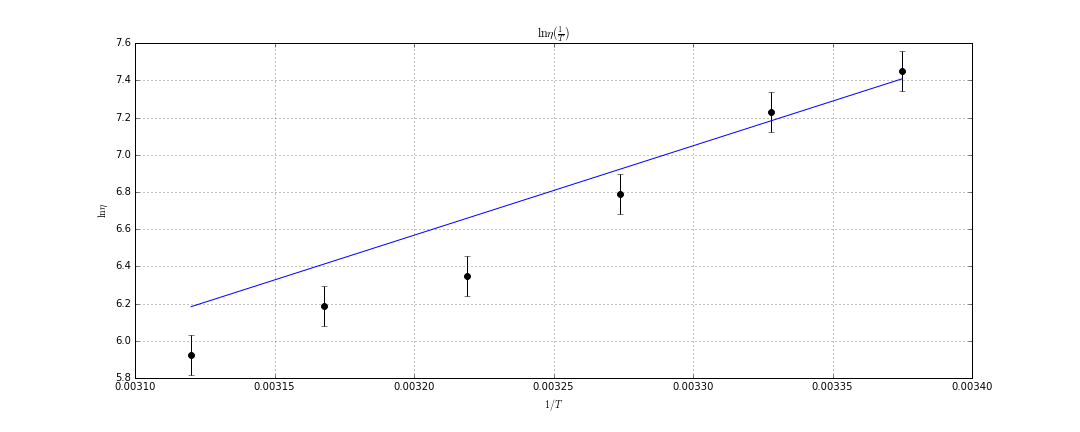
\includegraphics[width=18cm]{g2.png} 
    \end{center}

    $\sigma_{tg \alpha} = 293.5 , \varepsilon_{tg \alpha} = 0.05$ \\
    $\tg \alpha \approx 5906.8 \implies W = (8.16 \pm 0.40)* 10^{-20}$ [Дж] $\approx 0.51$ [эВ].

    При рассчитанной достаточно малой погрешности в $2 - 5 \%$, мы получили достаточно большую разницу результатов (около 12 - 14 \%). Это может говорить о том, что несферическая форма металлических шариков(для которых применима формула Стокса) внесла большую погрешность, чем мы учли. 

\end{enumerate}


\end{document}